\subsection{Reproduction of the Drude fits}
We could reproduce most of the results of Legros et al. (Figure \ref{fig:drude_fit_good}).
However, no matter how much we fine-tuned the fitting procedure, we could not produce fits looking
as good as theirs for some of the plots (Figure \ref{fig:drude_fit_bad}). So, we tried fitting the
real part and the imaginary part of the optical conductivity separately, and we could produce
similar-looking fits. Extracting the parameters from these fits and comparing them to the parameters
extracted from the fits of Legros et al., we found that the parameters were consistent. This leads
us to believe this is indeed what Legros et al. did in their analysis. 

Fitting the real and imaginary parts separately is not ``correct'' in some sense, but since the
imaginary part of the optical conductivity is dominated by a superconducting singularity, fitting
it separately can be a reasonable choice. This line of reasoning breaks down when there is not a
large singularity due to superconductivity, but most of these cases are well-fitted. There does
exist a few cases with small supercunductivity, but bad fits with simultaniously fitting the real
and imaginary parts of the optical conductivity, though.

To conclude, the fitting procedure of Legros et al. is badly documented and we cannot be completely
sure of their method. However, we could reproduce their results by fitting the real and imaginary
parts of the optical conductivity separately. This might be used as another objection to this paper,
but since we lack their full parameter output and details about their fitting procedure, we do not
assert that they definitly did this to ``fix'' their fits.

\begin{figure}
    \centering
    \begin{subfigure}{0.49\textwidth}
        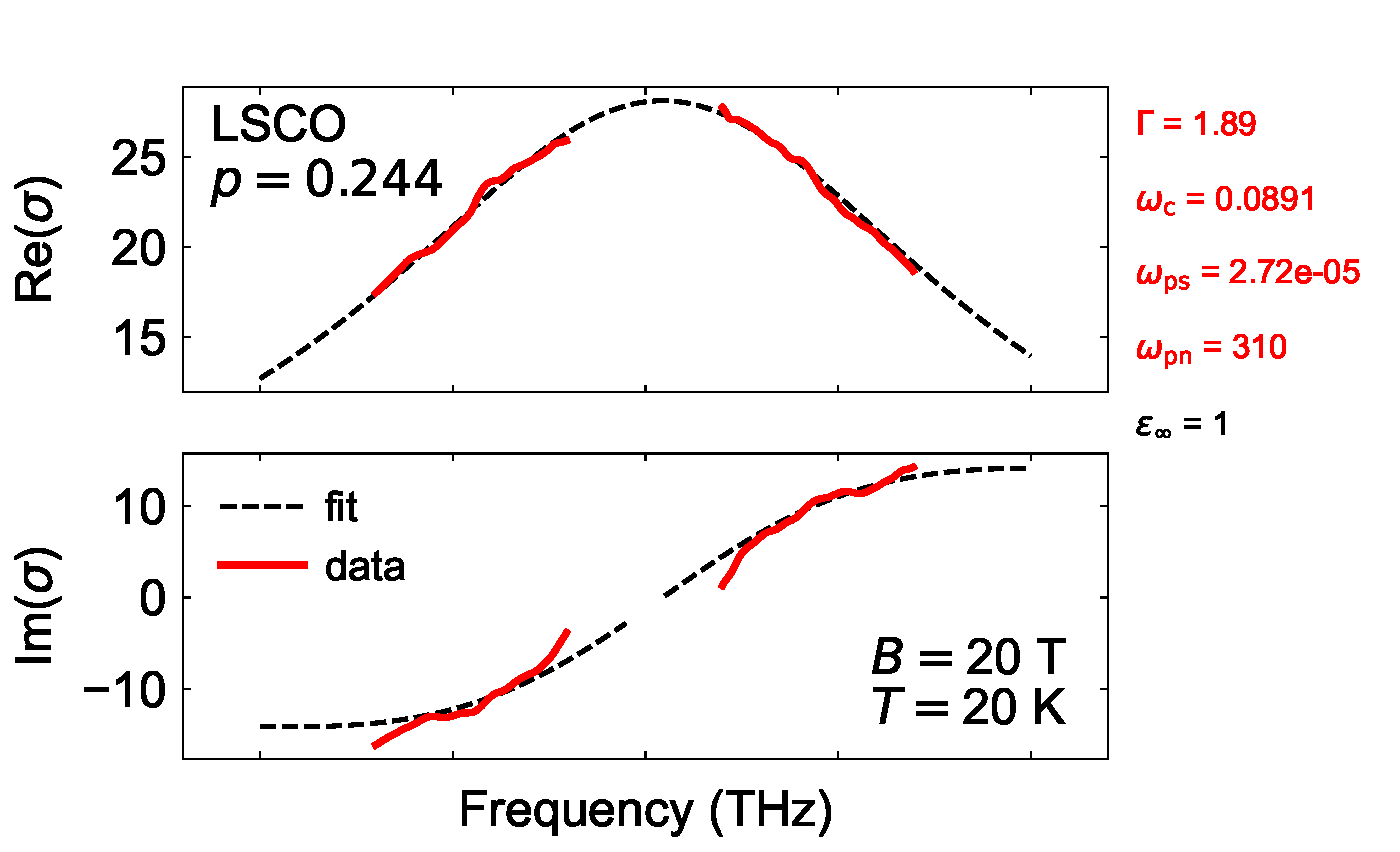
\includegraphics[width=\textwidth]{figures/drude_fit_good.pdf}
        \caption{A good fit while fitting the real and imaginary parts of the optical conductivity
            simultaneously.}
        \label{fig:drude_fit_good}
    \end{subfigure}
    \begin{subfigure}{0.5\textwidth}
        \centering
        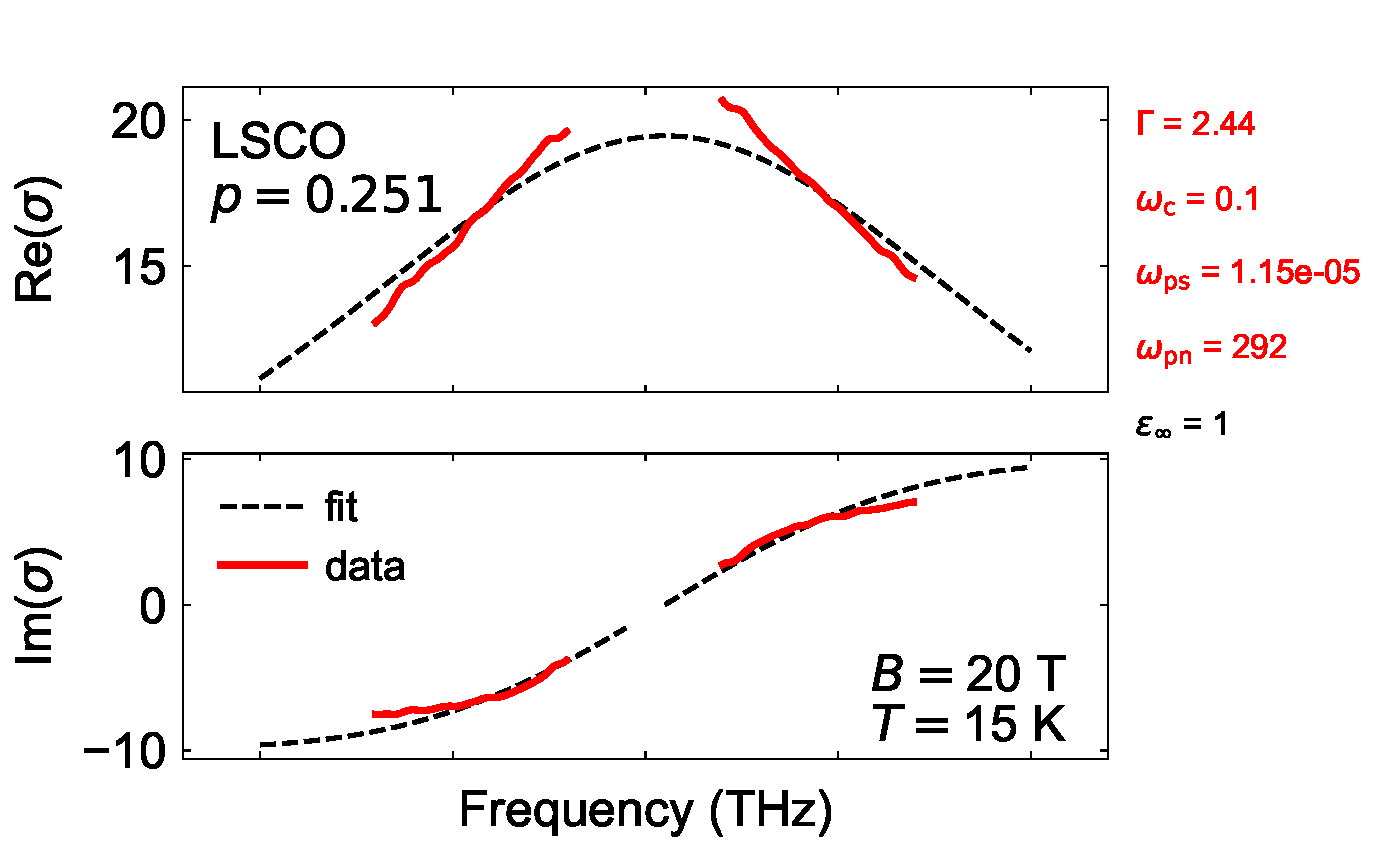
\includegraphics[width=\textwidth]{figures/drude_fit_bad.pdf}
        \caption{A bad fit while fitting the real and imaginary parts of the optical conductivity
            simultaneously.}
        \label{fig:drude_fit_bad}
    \end{subfigure}
    \begin{subfigure}{0.49\textwidth}
        \centering
        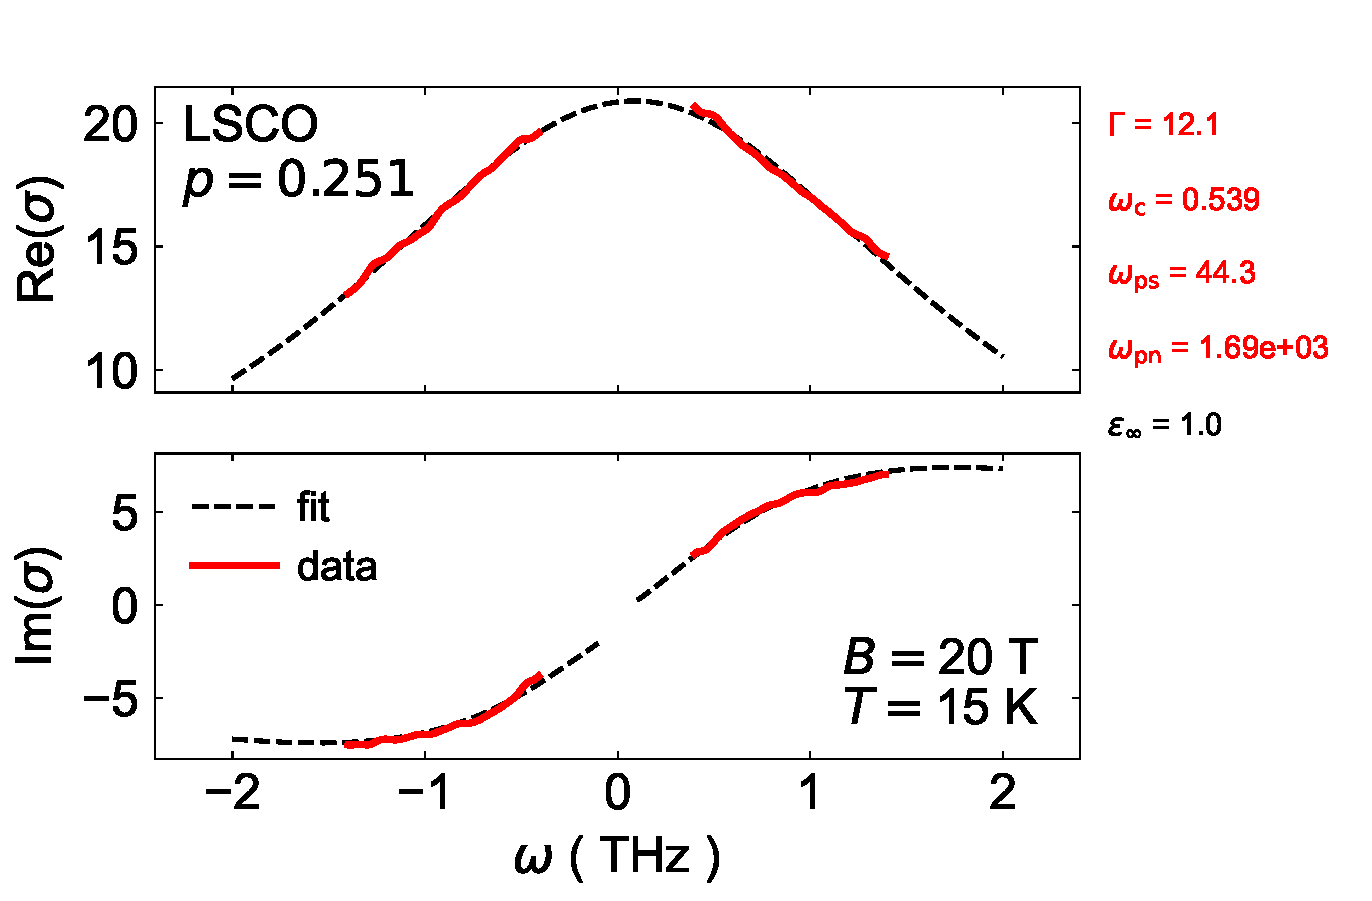
\includegraphics[width=\textwidth]{figures/drude_fit_fixed.pdf}
        \caption{A fit fixed by fitting the real and imaginary parts of the optical conductivity
            separately.}
        \label{fig:drude_fit_bad}
    \end{subfigure}
\end{figure}

%%% We can show the reproduction of Post et al. too maybe ?

\begin{figure}
    \centering
    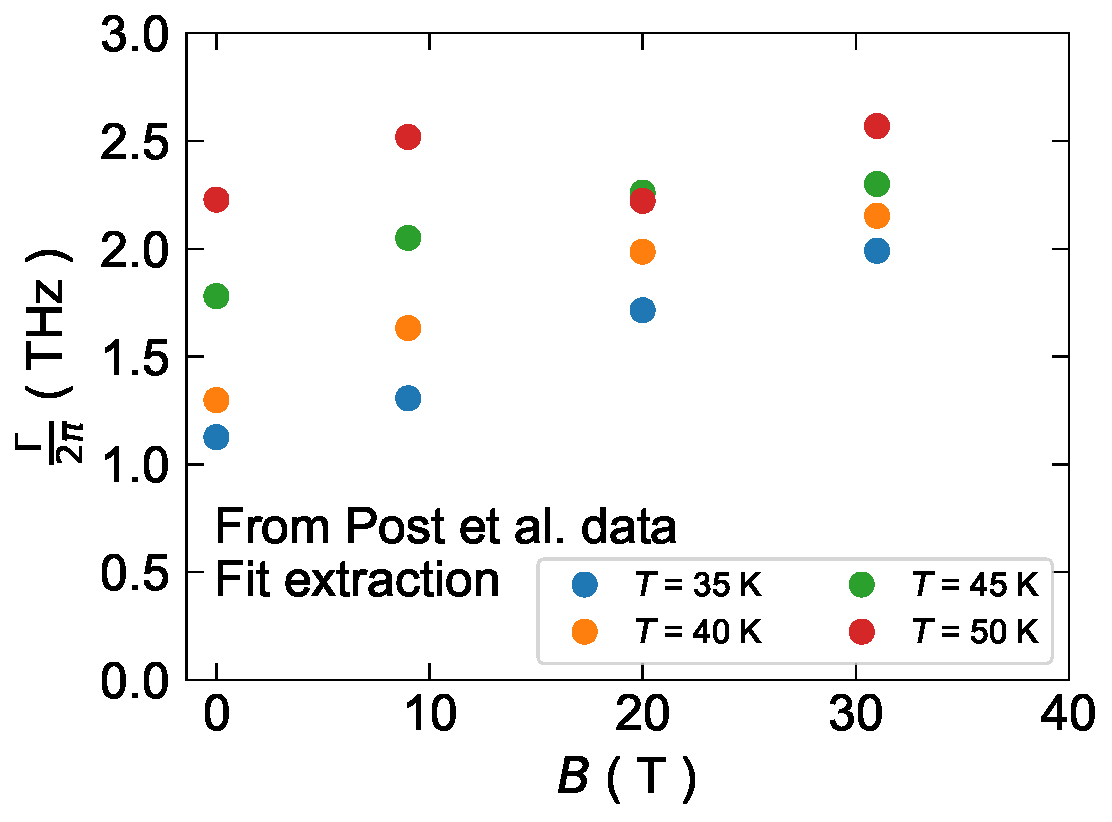
\includegraphics[width=0.7\textwidth]{figures/fitting_Drude_extracted_Gamma.pdf}
    \caption{ADD SUBFIGURE A comparison of our and their fits with their data}
    \label{fig:drude_fit_good}
\end{figure}
